%%
%% This is file `sample-sigplan.tex',
%% generated with the docstrip utility.
%%
%% The original source files were:
%%
%% samples.dtx  (with options: `all,proceedings,bibtex,sigplan')
%% 
%% IMPORTANT NOTICE:
%% 
%% For the copyright see the source file.
%% 
%% Any modified versions of this file must be renamed
%% with new filenames distinct from sample-sigplan.tex.
%% 
%% For distribution of the original source see the terms
%% for copying and modification in the file samples.dtx.
%% 
%% This generated file may be distributed as long as the
%% original source files, as listed above, are part of the
%% same distribution. (The sources need not necessarily be
%% in the same archive or directory.)
%%
%%
%% Commands for TeXCount
%TC:macro \cite [option:text,text]
%TC:macro \citep [option:text,text]
%TC:macro \citet [option:text,text]
%TC:envir table 0 1
%TC:envir table* 0 1
%TC:envir tabular [ignore] word
%TC:envir displaymath 0 word
%TC:envir math 0 word
%TC:envir comment 0 0
%%
%% The first command in your LaTeX source must be the \documentclass
%% command.
%%
%% For submission and review of your manuscript please change the
%% command to \documentclass[manuscript, screen, review]{acmart}.
%%
%% When submitting camera ready or to TAPS, please change the command
%% to \documentclass[sigconf]{acmart} or whichever template is required
%% for your publication.
%%
%%
% !TEX root = main.tex
\documentclass[sigplan,screen]{acmart}
\usepackage{graphicx} 
\usepackage{caption} 
\usepackage{float}
\usepackage{amsmath}

%%
%% \BibTeX command to typeset BibTeX logo in the docs
\AtBeginDocument{%
  \providecommand\BibTeX{{%
    Bib\TeX}}}
  
%% Rights management information.  This information is sent to you
%% when you complete the rights form.  These commands have SAMPLE
%% values in them; it is your responsibility as an author to replace
%% the commands and values with those provided to you when you
%% complete the rights form.
\setcopyright{acmlicensed}
\copyrightyear{2018}
\acmYear{2018}
\acmDOI{XXXXXXX.XXXXXXX}
%% These commands are for a PROCEEDINGS abstract or paper.
\acmConference[Conference acronym 'XX]{Make sure to enter the correct
  conference title from your rights confirmation emai}{June 03--05,
  2018}{Woodstock, NY}
%%
%%  Uncomment \acmBooktitle if the title of the proceedings is different
%%  from ``Proceedings of ...''!
%%
%%\acmBooktitle{Woodstock '18: ACM Symposium on Neural Gaze Detection,
%%  June 03--05, 2018, Woodstock, NY}
\acmISBN{978-1-4503-XXXX-X/18/06}


%%
%% Submission ID.
%% Use this when submitting an article to a sponsored event. You'll
%% receive a unique submission ID from the organizers
%% of the event, and this ID should be used as the parameter to this command.
%%\acmSubmissionID{123-A56-BU3}

%%
%% For managing citations, it is recommended to use bibliography
%% files in BibTeX format.
%%
%% You can then either use BibTeX with the ACM-Reference-Format style,
%% or BibLaTeX with the acmnumeric or acmauthoryear sytles, that include
%% support for advanced citation of software artefact from the
%% biblatex-software package, also separately available on CTAN.
%%
%% Look at the sample-*-biblatex.tex files for templates showcasing
%% the biblatex styles.
%%

%%
%% The majority of ACM publications use numbered citations and
%% references.  The command \citestyle{authoryear} switches to the
%% "author year" style.
%%
%% If you are preparing content for an event
%% sponsored by ACM SIGGRAPH, you must use the "author year" style of
%% citations and references.
%% Uncommenting
%% the next command will enable that style.
%%\citestyle{acmauthoryear}


%%
%% end of the preamble, start of the body of the document source.
\begin{document}
\small
%%
%% The "title" command has an optional parameter,
%% allowing the author to define a "short title" to be used in page headers.
\title{The Name of the Title Is Hope}

%%
%% The "author" command and its associated commands are used to define
%% the authors and their affiliations.
%% Of note is the shared affiliation of the first two authors, and the
%% "authornote" and "authornotemark" commands
%% used to denote shared contribution to the research.
\author{Gavin Ji}
\affiliation{%
 \institution{University of California, San Diego}}
 
\author{Aaron Ang}
\affiliation{%
 \institution{University of California, San Diego}}

% \email{larst@affiliation.org}


\author{Jiangrong Liu}
\affiliation{%

 \institution{University of California, San Diego}}


\author{Lingfeng Ma}
\affiliation{%
  \institution{University of California, San Diego}}
  



%%
%% By default, the full list of authors will be used in the page
%% headers. Often, this list is too long, and will overlap
%% other information printed in the page headers. This command allows
%% the author to define a more concise list
%% of authors' names for this purpose.
\renewcommand{\shortauthors}{Trovato et al.}

%%
%% The abstract is a short summary of the work to be presented in the
%% article.
\begin{abstract}
  A clear and well-documented \LaTeX\ document is presented as an
  article formatted for publication by ACM in a conference proceedings
  or journal publication. Based on the ``acmart'' document class, this
  article presents and explains many of the common variations, as well
  as many of the formatting elements an author may use in the
  preparation of the documentation of their work.
\end{abstract}

%%
%% The code below is generated by the tool at http://dl.acm.org/ccs.cfm.
%% Please copy and paste the code instead of the example below.
%%
\begin{CCSXML}
<ccs2012>
 <concept>
  <concept_id>00000000.0000000.0000000</concept_id>
  <concept_desc>Do Not Use This Code, Generate the Correct Terms for Your Paper</concept_desc>
  <concept_significance>500</concept_significance>
 </concept>
 <concept>
  <concept_id>00000000.00000000.00000000</concept_id>
  <concept_desc>Do Not Use This Code, Generate the Correct Terms for Your Paper</concept_desc>
  <concept_significance>300</concept_significance>
 </concept>
 <concept>
  <concept_id>00000000.00000000.00000000</concept_id>
  <concept_desc>Do Not Use This Code, Generate the Correct Terms for Your Paper</concept_desc>
  <concept_significance>100</concept_significance>
 </concept>
 <concept>
  <concept_id>00000000.00000000.00000000</concept_id>
  <concept_desc>Do Not Use This Code, Generate the Correct Terms for Your Paper</concept_desc>
  <concept_significance>100</concept_significance>
 </concept>
</ccs2012>
\end{CCSXML}

\ccsdesc[500]{Do Not Use This Code~Generate the Correct Terms for Your Paper}
\ccsdesc[300]{Do Not Use This Code~Generate the Correct Terms for Your Paper}
\ccsdesc{Do Not Use This Code~Generate the Correct Terms for Your Paper}
\ccsdesc[100]{Do Not Use This Code~Generate the Correct Terms for Your Paper}

%%
%% Keywords. The author(s) should pick words that accurately describe
%% the work being presented. Separate the keywords with commas.
\keywords{Do, Not, Us, This, Code, Put, the, Correct, Terms, for,
  Your, Paper}
%% A "teaser" image appears between the author and affiliation
%% information and the body of the document, and typically spans the
%% page.
\begin{teaserfigure}
  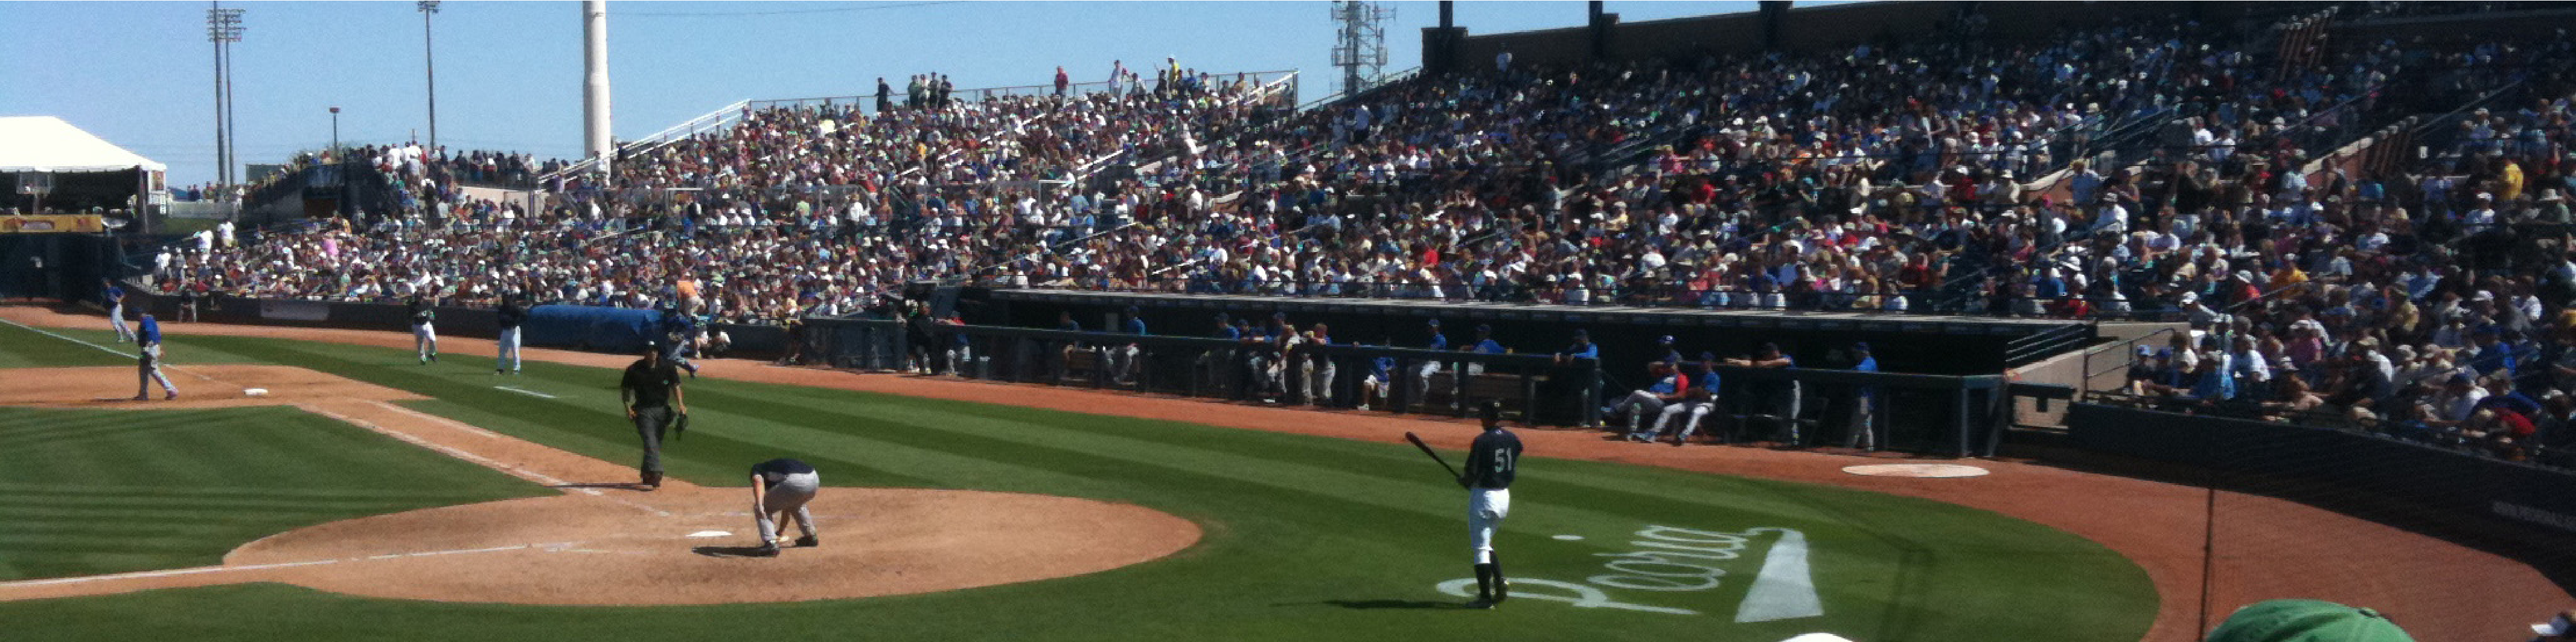
\includegraphics[width=\textwidth]{sampleteaser}
  \caption{Seattle Mariners at Spring Training, 2010.}
  \Description{Enjoying the baseball game from the third-base
  seats. Ichiro Suzuki preparing to bat.}
  \label{fig:teaser}
\end{teaserfigure}

\received{20 February 2007}
\received[revised]{12 March 2009}
\received[accepted]{5 June 2009}

%%
%% This command processes the author and affiliation and title
%% information and builds the first part of the formatted document

\section{Data Exploring}
The "Trending YouTube Video Statistics" is selected as the dataset \cite{daatset}. In general, the dataset focus on daily records of trending viedos on Youtube. It consists of informations of trending viedos in 10 countries (USA, Great Britain, Germany, Canada, France, Russia, Mexico, South Korea, Japan and India). Entries from each country are stored in a CSV file. For each entry, the video title, channel title, publish time, tags, views, likes and dislikes, description, and comment count are recorded, where video title, channel title, tags and description are text and others are digits. Among them, the title, tags, description, views, likes, dislikes and comment count are selected for further tasks.

\subsection{Distributions of numerical data}
The distributions of all numerical data in the dataset are obtained and those distributions of different countries shares similarity. 
\begin{table}[ht]
  \centering
  \caption{Descriptive Statistics of Video Metrics (CA)}
  \label{tab:video_metrics}
  \begin{tabular}{lccccc}
  \toprule
  \textbf{Statistic} & \textbf{Views} & \textbf{Likes} & \textbf{Dislikes} & \textbf{Comment Count} \\
  \midrule
  Count & 39,585 & 39,585 & 39,585 & 39,585 \\
  Mean & 1,169,234.01 & 40,596.94 & 2,058.69 & 5,159.72 \\
  Std. Dev. & 3,437,842.10 & 134,596.73 & 19,312.58 & 21,899.59 \\
  Min & 733 & 0 & 0 & 0 \\
  25\% & 149,715 & 2,395 & 104 & 442 \\
  Median & 383,120 & 9,244 & 314 & 1,357 \\
  75\% & 983,139 & 29,670 & 976 & 3,821 \\
  Max & 137,843,120 & 5,053,338 & 1,602,383 & 1,114,800 \\
  \bottomrule
  
  \end{tabular}
  \end{table}

According to Table \ref{tab:video_metrics}, the basic statistics information of numerical data in Canada is provided. Both the mean and median values of views are much larger than those of likes, dislikes and comment count. Additionally, the standard deviations of all metrics are larger than their mean but smaller than ten times of the mean, which means their distributions are dispersive, such as the exponential distribution.

For each numerical metrics, their distributions are generated and the distributions in Canada are provided. And the probability distribution functions (PDF) obtained fromstimation (KDE) kernel density and exponential fitting are used. According to Figure \ref{fig:views}, Figure \ref{fig:likes}, Figure \ref{fig:dislikes}, Figure \ref{fig:comments}, their distributions are exponential distributions, meaning that most of the data are small and close with few extremely high data. Therefore, all numerical data are preprocessed into log-scale in further tasks to ensure the models to converge.

\begin{figure}[H]
  \centering
  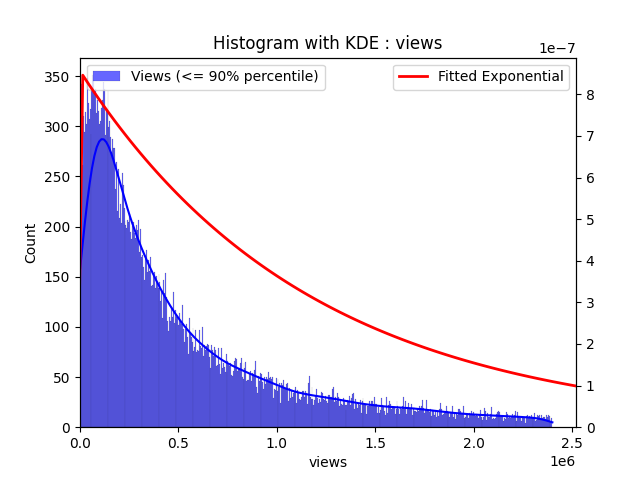
\includegraphics[width=0.6\textwidth]{figure/CAviewsDistrbution.png} 
  \caption{The distribution of views in Canada. The PDFs generated form KDE and exponential fitting are used. The max 10\% data are ignored.}
  \label{fig:views} 
  \end{figure}
  \begin{figure}[H]
    \centering
    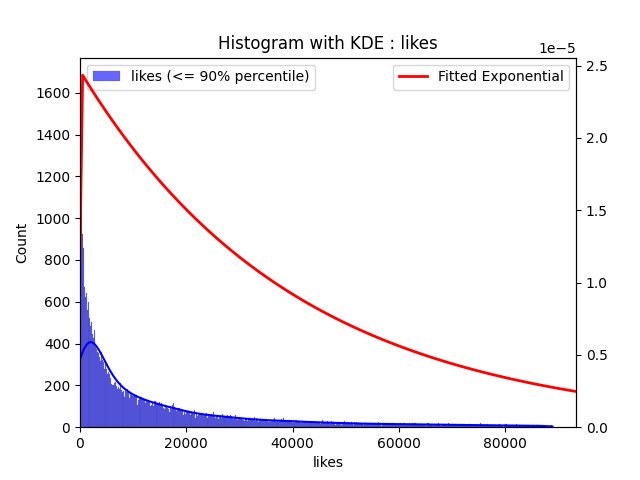
\includegraphics[width=0.6\textwidth]{figure/CAlikesDistrbution.png} 
    \caption{The distribution of likes in Canada. The PDFs generated form KDE and exponential fitting are used. The max 10\% data are ignored.}
    \label{fig:likes} 
    \end{figure}
    \begin{figure}[H]
      \centering
      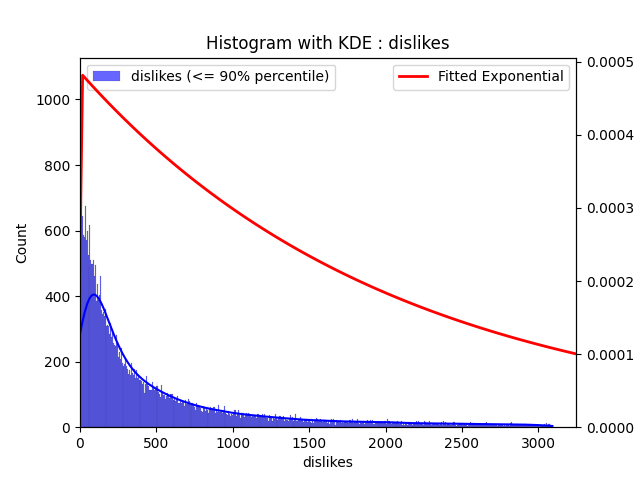
\includegraphics[width=0.6\textwidth]{figure/CAdislikesDistrbution.png} 
      \caption{The distribution of dislikes in Canada. The PDFs generated form KDE and exponential fitting are used. The max 10\% data are ignored.}
      \label{fig:dislikes} 
      \end{figure}
      \begin{figure}[H]
        \centering
        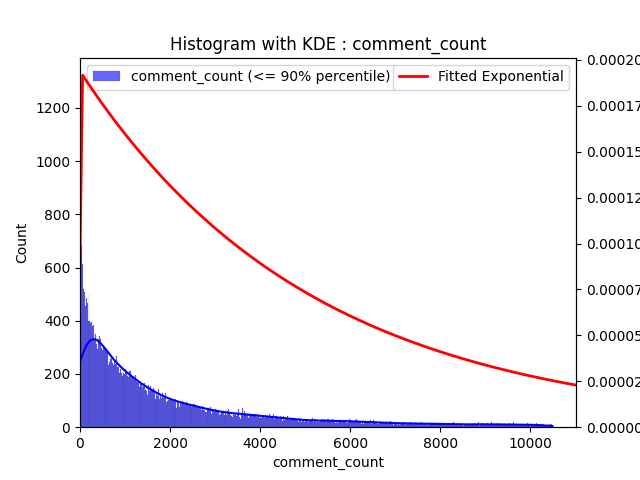
\includegraphics[width=0.6\textwidth]{figure/CAcomment_countDistrbution.png} 
        \caption{The distribution of comments count in Canada. The PDFs generated form KDE and exponential fitting are used. The max 10\% data are ignored.}
        \label{fig:comments} 
        \end{figure}
\subsection{Word Frequency}

The frequency of words in the text data provided signification information about the video. After removing the irrelevant informations such as stopping words and urls, the word frequency of title, tags and descriptions are generated as the word clouds.
\begin{figure}[H]
  \centering
  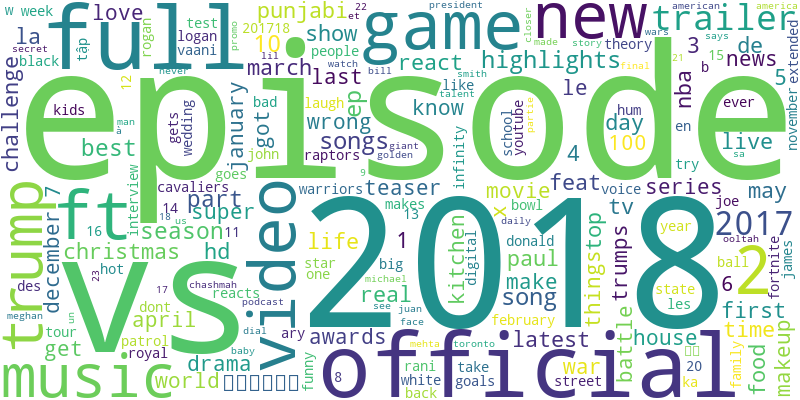
\includegraphics[width=0.6\textwidth]{figure/CAtitleWordCloud.png} 
  \caption{The word cloud of titles in Canada.}
  \label{fig:title} 
\end{figure}
\begin{figure}[H]
  \centering
  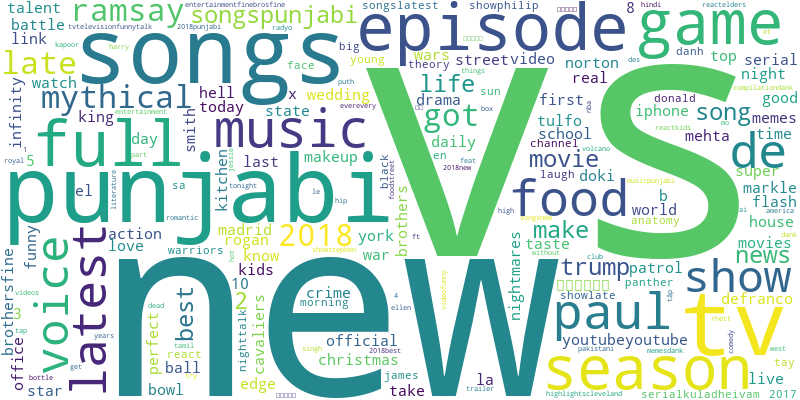
\includegraphics[width=0.6\textwidth]{figure/CAtagsWordCloud.png}
  \caption{The word cloud of tags in Canada.}
  \label{fig:tag} 
\end{figure}
\begin{figure}[H]
  \centering
  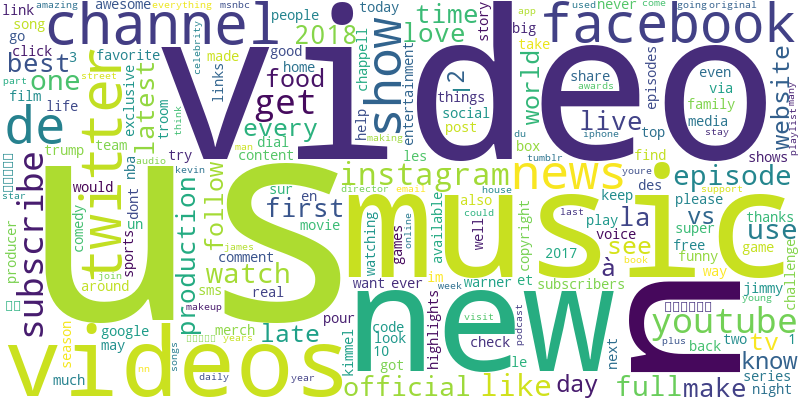
\includegraphics[width=0.6\textwidth]{figure/CAdescriptionWordCloud.png} 
  \caption{The word cloud of descriptions in Canada.}
  \label{fig:description} 
\end{figure}

\section{Task}
Since all features selected are expected to share strong releations, each feature can be potentialy predicted by other features. Taking consideration of the real world application, the prediction of views of a viedo is selected as the task. Since views of a viedo can significantly indicate its popularity, the effective prediction can direct the creators while improve the recommendation methods of platforms.

As the prediction target is views, a regression model is expected. Initially, the simple logistic regression models with other numerical features such as likes, dislikes and comment count is selected as baselines. Further, the Term Frequency-Inverse Document Frequency (TF-IDF) approach is expected to perform well with text features, such as titles, tags and descriptions. The MSE, MAE and $R^2$ are selected for evaluation.

All numerical features are converted into log-scale and all text features are preprocessed by removing irrelevant informations.



\section{Model}
To predict the views of a viedo, all other metrics in the entry can be considered as features. Since the views, likes, dislikes and comment count share the same distributions, the regression models using likes, dislikes and comment count as inputs are expected to perfomr well. However, the prediction task can not be actually completed with these models since the views data is available if likes, dislikes and comment count are available. And using features to predict an existed data is meaningless.

The title, tags and descriptions of a viedo are available once it is uploaded. Therefore, these informations can be applied as features for prediction. Then the TF-IDF approach can be used, which provides the contribution of a word to text. The word with higher frequency in a sample text and lower frequency in the whole text is assigned with higher weight, and vice versa. The method focus on the releation between each signle word and the sample text. However, the context information is aborted and all words are considered as independent.

Introduced by \cite{NIPS2017_3f5ee243}, the self-attention based approach : Transformer, is proven to perform well in processing texts. It weights the importance of releations among different words, enabling it to extract the context and global information. In general, the model develops the encoder-decoder structure. In the encoder, inputs are converted into tokens, which are the minimum units of information. Then, linear layers are applied to map the input tokens into three matrixes: Query, Key and Value. And the attention weights are generated by the matrixes.
\[
\text{Attention}(Q, K, V) = \text{softmax}\left(\frac{QK^T}{\sqrt{d_k}}\right)V
\]
In the decoder, a prediction head is used to generate the prediction result from the weights.

To apply Transformer in the views prediction task, the features (title, tags and descriptions) are converted into tokens, which are the basic unit of the text. After that, a pre-trained Transformer model with signle head is adopted. In each epoch of training, the model's performance on the validation set is evaulated and early-stopping is adopted to avoid overfitting.

\section{Literature}

Similar prediction tasks are completed with the dataset, such as likes prediction, Category Prediciton \cite{likespred,categorypred}

Although Transformer based approach archives the best performance, it is limited by huge time and space consumption since each token has interactions with all tokens. Although its self-attention mechanism can obtain the context information, the computation cost increases rapidly as the text seqence increasing. The Receptance-Weighted Key-Value (RWKV) model combines the RNN and self-attention, archives high performance on large scale tasks with acceptable costs \cite{peng2023rwkvreinventingrnnstransformer}. Its RNN structure reduces the time and space consumption and its time decay mechanism performs well on processing long scale information.

\section{Experiments and Results}
\begin{table}[H]
  \centering
  
  \caption{Performance Metrics of Models}
  \label{tab:model_metrics}
 
  \begin{tabular}{lccc}
  \toprule
  \textbf{Model} & \textbf{MSE} & \textbf{MAE} & \textbf{$R^2$} \\
  \midrule
  Single Feature (likes) & 0.77 & 0.63 & 0.74 \\
  Single Feature (comments) & 1.19 & 0.77 & 0.60 \\
  Single Feature (dislikes) & 0.76 & 0.64 & 0.74 \\
  TF-IDF (tags) & 0.43 & 0.33 & 0.86 \\
  TF-IDF-SVD (tags) & 1.27 & 0.42 & \bf{0.58} \\
  TF-IDF (description) & 0.80 & 0.31 & 0.74 \\
  TF-IDF-SVD (description) & 0.55 & 0.39 & 0.82 \\
  TF-IDF (title) & 0.32 & 0.28 & 0.89 \\
  TF-IDF-SVD (title) & 0.44 & 0.38 & 0.85 \\
  Transformer (tags) & 0.44 & 0.38 & 0.85 \\
  Transformer (description) & 0.30 & 0.35 & 0.90 \\
  Transformer (title) & \bf{0.18} & \bf{0.27} & 0.93 \\
  \bottomrule
  \end{tabular}%
  
\end{table}

Table \ref{tab:model_metrics} provides the performance of 12 different models. The dataset is likes, comments, dislikes, tags, description and titles in US, with size of 40739. After shuffle, 90\% of the dataset is devided as the training set and 10\% is the validation set. The metrics of MSE, MAE and $R^2$ are used.

The baselines are in three groups: regression models with signle features, TF-IDF models and TF-IDF-SVD models. For TF-IDF models, the max 20000 imprtant words are used. For TF-ID-SVD models, the Singular Value Decomposition approach is introduced for dimension reduction from 20000 to 5000.

As the result, the Transformer model with titles as features archives the best performance: 0.18 in MSE and 0.27 in MAE, proving the effectiveness of Transformer on texts prediction tasks. Furthermore, all models with titles perform better than other text features, indicating that the title of a video contributes more with its views than tags and descriptions.




%%
%% The acknowledgments section is defined using the "acks" environment
%% (and NOT an unnumbered section). This ensures the proper
%% identification of the section in the article metadata, and the
%% consistent spelling of the heading.
\begin{acks}
To Robert, for the bagels and explaining CMYK and color spaces.
\end{acks}

%%
%% The next two lines define the bibliography style to be used, and
%% the bibliography file.
\bibliographystyle{ACM-Reference-Format}
\bibliography{sample-base}


%%
%% If your work has an appendix, this is the place to put it.
\appendix

\section{Research Methods}

\subsection{Part One}

Lorem ipsum dolor sit amet, consectetur adipiscing elit. Morbi
malesuada, quam in pulvinar varius, metus nunc fermentum urna, id
sollicitudin purus odio sit amet enim. Aliquam ullamcorper eu ipsum
vel mollis. Curabitur quis dictum nisl. Phasellus vel semper risus, et
lacinia dolor. Integer ultricies commodo sem nec semper.

\subsection{Part Two}

Etiam commodo feugiat nisl pulvinar pellentesque. Etiam auctor sodales
ligula, non varius nibh pulvinar semper. Suspendisse nec lectus non
ipsum convallis congue hendrerit vitae sapien. Donec at laoreet
eros. Vivamus non purus placerat, scelerisque diam eu, cursus
ante. Etiam aliquam tortor auctor efficitur mattis.

\section{Online Resources}

Nam id fermentum dui. Suspendisse sagittis tortor a nulla mollis, in
pulvinar ex pretium. Sed interdum orci quis metus euismod, et sagittis
enim maximus. Vestibulum gravida massa ut felis suscipit
congue. Quisque mattis elit a risus ultrices commodo venenatis eget
dui. Etiam sagittis eleifend elementum.

Nam interdum magna at lectus dignissim, ac dignissim lorem
rhoncus. Maecenas eu arcu ac neque placerat aliquam. Nunc pulvinar
massa et mattis lacinia.

\end{document}
\endinput
%%
%% End of file `sample-sigplan.tex'.
